\begin{block}{Distribution Estimation}
\centering
        \heading{Goal: Obtain the Best Distribution of $\lambda$} 
            {\large \textbf{Bayesian Context:} Simple Bayes model is insufficient, hierarchical Bayes model required.}
           
           {\large \textbf{Data Consistent Context:} Use data to construct observed distribution.}
           
           {\large \  }

        %\heading{Background}
             %{\large \emph{Data Consistent Inversion} is a Measure-Theoretic Framework for the solution of stochastic inverse problems. }
             
\end{block}

\vspace{-0.75cm}
\begin{block}{Example}
\centering
Consider an exponential decay problem with uncertain decay rate:
\begin{equation*}
       u(t) = u_0\exp(-\lambda t), \; u_0 = 0.5 ,\; t=2
   \end{equation*}

\begin{tabular}{c|c}
\hline
\multirow{2}{*}{\vspace{1.5ex}\textbf{Simple Bayes}} & 
$\begin{aligned}\prior \sim U[0,1]\; , \quad  \likelihood\qGivelam\sim N\left(Q\lam,\sigma^2\right) \end{aligned}$ \\[1.25ex]
                                        & $\bayes$ \\
\hline
\multirow{2}{*}{\vspace{2ex} \textbf{Hierarchical Bayes}}   & $\begin{aligned}
        \prior\hyper &\sim \chi^2_1\; , \quad \alpha,\beta\in\Omega:=[0,\infty)\times[0,\infty) \\[1.25ex]
        \prior\lamGiveH &\sim \text{Beta}\hyper \\[1.25ex]
        \likelihood\qGivelam &\sim N\left(Q\lam,\sigma^2\right)\\[1.25ex] \end{aligned}$ \\[1.25ex]
                                    & $\Hbayes$ \\
\hline
\textbf{Data Consistent} &  $\dci$ \\
\hline
\end{tabular}
\vspace{1cm}
\heading{Plots of Concepts and Results}
% \begin{figure}
%         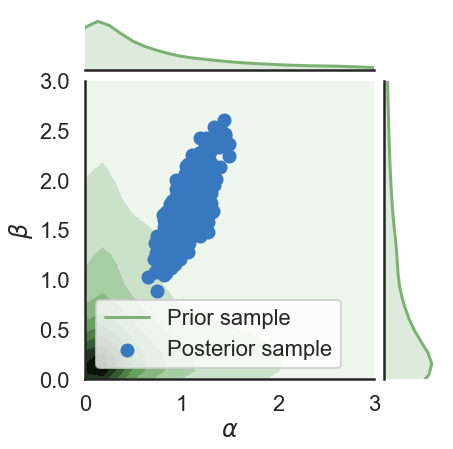
\includegraphics[width=10cm]{figures/distr_EX_hyper_param.png}
%         \vspace{-0.5cm}
%         \caption{$hyperspace$}
% \end{figure}
%\vspace{-1cm}
\begin{figure}
        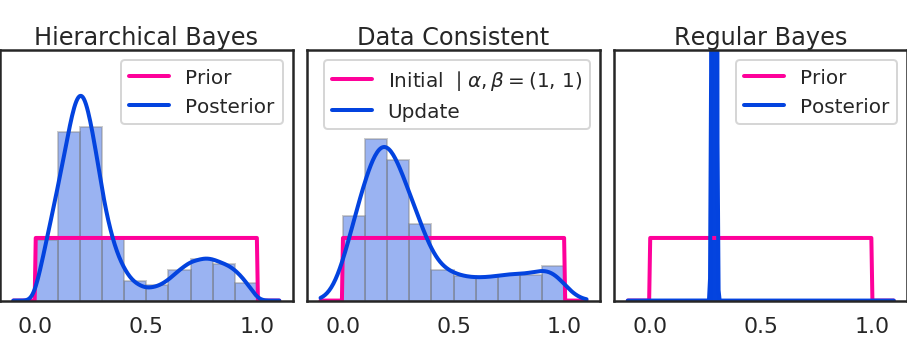
\includegraphics[width=32cm]{figures/distr_EX_lambda_space.png}
        \vspace{-0.5cm}
        \centering
        \caption{\large $\pspace$ Parameter Space }
\end{figure}
\vspace{-0.5cm}
\begin{figure}
        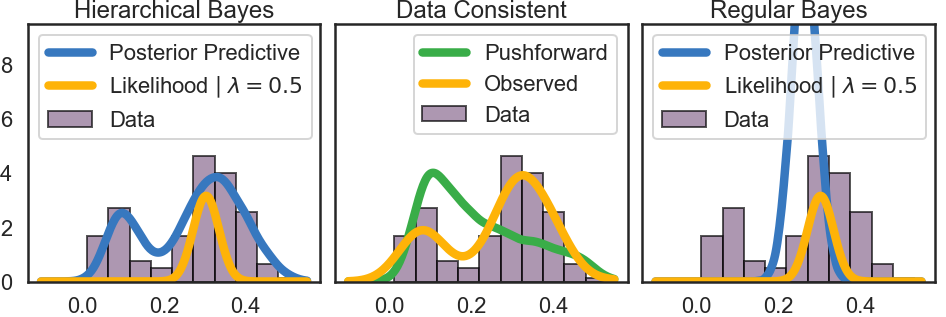
\includegraphics[width=32cm]{figures/distr_EX_data_space.png}
        \vspace{-0.5cm}
        \centering
        \caption{\large $\dspace$ Parameter Space  }
\end{figure}


\end{block}


\vspace{-1.cm}


\begin{block}{Takeaways}

\centering
    \heading{Non-parametric method with less sampling}
%     \begin{equation*}
%             \dciP \quad \vline \quad \dci
%     \end{equation*}
    %\begin{equation*}
    %        \dci
    %\end{equation*}
\vspace{-0.5cm}
\begin{figure}
        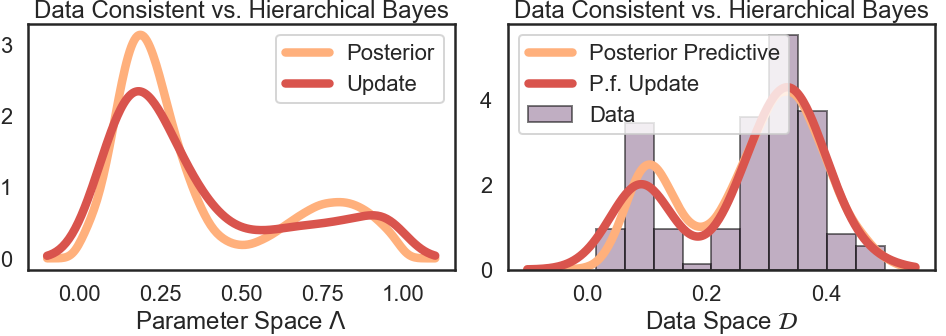
\includegraphics[width=30cm]{figures/distr_EX_comparison.png}
        \vspace{-0.5cm} 
        \caption{ }
    \end{figure}
\end{block}
%\textbf{Future research:} What are the connections to Dirchlet processes?
